\section{Tour / examples}
\label{sec:tour}

\newpage



\vspace{2em}
example - 2

% Second row
\noindent
\begin{minipage}[t]{0.45\textwidth}
	\begin{lstlisting}[caption={Not serializable: {(A,0),(A,0)}}]
			request A: 
			    x := FLAG 
			
			    if (?): 
			        yield
			    // no else
			
			
			    FLAG := 1 
			    return x
		\end{lstlisting}
\end{minipage}%
\hfill
\begin{minipage}[t]{0.45\textwidth}
	\begin{lstlisting}[caption={Serializable}]
			request A: 
			    x := FLAG
			
			    if (?):
			        yield
			    else:
			        x := 1 - x
			
			    FLAG := 1
			    return x
		\end{lstlisting}
\end{minipage}

\vspace{2em}
%\newpage
example - 3

% Third row
\noindent
\begin{minipage}[t]{0.45\textwidth}
	\begin{lstlisting}[caption={Fred (serializable)}]
			request incr: 
			    while (X == 3):
			        yield
			        
			        
			    X := X + 1
				  return X		
			
			request decr: 
			    while (X == 0): 
			        yield
			        
			        
			    X := X - 1
				  return X
		\end{lstlisting}
\end{minipage}
\hfill
\begin{minipage}[t]{0.45\textwidth}
	\begin{lstlisting}[caption={Fred2 (not serializable)}]
			request incr:
			    while (X == 3):
			        yield
			    y := X
			    yield
			    X := y + 1
		      return X		
			
			request decr: 
			    while (X == 0):
			        yield
			    y := X
			    yield
			    X := y - 1
		      return X
		\end{lstlisting}
\end{minipage}
	
\newpage

example - 4

\begin{minipage}[t]{1.0\textwidth}
\begin{lstlisting}[caption={Snapshot-based monitor deactivation (not serializable, as it can return a sume of 0 active monitors)}]
	// initialize both monitors to be active
    N_1_ACTIVE := 1
    N_2_ACTIVE := 1
	
    request main:
        // take snapshot
        n_1_active_snapshot := N_1_ACTIVE
        n_2_active_snapshot := N_2_ACTIVE
        yield
		
        if (n_1_active_snapshot == 1) and (n_2_active_snapshot == 1):
            // if both nodes active --- choose which one to deactivate 
            if (?): 
                N_1_ACTIVE := 0
            else:
                N_2_ACTIVE := 0

        return N_1_ACTIVE + N_2_ACTIVE  // total active nodes
        
        
        request activate_n1:
        	N_1_ACTIVE := 1
        
        request activate_n2:
        	N_2_ACTIVE := 1
        
        
\end{lstlisting}
\end{minipage}
	
%only 0 in non-serializable runs!

%\todo{start}

%/snapshot_isolation_directly_as_NS_with_yields

\begin{figure}[h]
	\centering
\includegraphics[width=1.0\linewidth]{plots/snapshot\_isolation\_JSON\_with\_yields.pdf}
	\caption{Snapshot Isolation with Yields.}
	\label{fig:snapshotIsolationJsonWithYields}
\end{figure}



%/snapshot_isolation_directly_as_NS_without_yields

\begin{figure}[h]
	\centering
	\includegraphics[width=1.0\linewidth]{plots/snapshot\_isolation\_JSON\_without\_yields.pdf}
	\caption{Snapshot Isolation with Yields.}
	\label{fig:snapshotIsolationJsonWithoutYields}
\end{figure}


\todo{maybe we have: (1) a copy of the global automaton; (2) a copy of the local automaton (with yields) with coloring of edges that don't exist in the one without yields}


\newpage

example - 5

\noindent
\begin{minipage}[t]{0.45\textwidth}
	\begin{lstlisting}[caption={bank (serializable)}]
	    // initialize accounts
	    A := 100
	    B := 50
	    
	    request transfer: 
	        // transfer 50$
	        A := A - 50
	        // no yield
	        B := B + 50
	        return A + B
				
	    request interest: 
	        // add a 100% interest
	        A := A + A
	        // no yield
	        B := B + B
	        return A + B	      		        
			\end{lstlisting}
\end{minipage}
\hfill
\begin{minipage}[t]{0.45\textwidth}
	\begin{lstlisting}[caption={bank with yields (non serializable)}]
	    // initialize accounts
	    A := 100
	    B := 50
			
	    request transfer: 
	        // transfer 50$
	        A := A - 50
	        yield
	        B := B + 50
	        return A + B
	
	    request interest: 
	        // add a 100% interest
	        A := A + A
	        yield
	        B := B + B
	        return A + B	      		        
		\end{lstlisting}
\end{minipage}
	
%\newpage


example - 6


% Second row
\noindent
\begin{minipage}[t]{0.45\textwidth}
	\begin{lstlisting}[caption={Complex while (serializable)}]
	    request flip: 
	        X := 1 - X 
	    
	    request main:
	        i := 5
	        while (i > 0):
	            while (X == 0):
	                pass
	            while (X == 1):
	                pass
	            i := i - 1
	        
	        return 1       
			\end{lstlisting}
\end{minipage}%
\hfill
\begin{minipage}[t]{0.45\textwidth}
	\begin{lstlisting}[caption={Complex while with yields (not serializable)}]
	    request flip: 
	        X := 1 - X 
	
	    request main:
	        i := 5
	        while (i > 0):
	            while (X == 0):
	                yield
	            while (X == 1):
	                yield
	            i := i - 1
	
	        return 1        
				\end{lstlisting}
\end{minipage}



\newpage

example - 7

\begin{minipage}[t]{1.0\textwidth}
	\begin{lstlisting}[caption={BGP (non serializable --- cycles can appear)}]
	    // initialize accounts
	    G := 0
	    
	    request policy_update:
	    if (?):
	        G := 1  // green policy 
	    else:
	        G := 0 // red policy
			
	    request route_from_west:
	        visited_east := 0
	        current := 1
	        while (current == 2) or (current == 3): // still routing        
	            if (current == 1): // west (switch 1)
	                if (G == 1): // green policy
	                    current := 2
	                else: // red policy
	                    current := 1
	            if (current == 2): // east (switch 2)
	                visited_east := 1
	                if (G == 1): // green policy
	                    current := 3
	                else: // red policy
	                    current := 1
	 
	            yield
			
	        return current + current + visited_east
	        
	    request route_from_east:
	        ... // dual case     		        
		\end{lstlisting}
\end{minipage}


%// [WEST, switch 1] ---> [EAST, switch 2] ---> [out, switch 3] 
%else:
%G := 0 // red policy
%// [out, switch 0] <--- [WEST, switch 1] <--- [EAST, switch 2] 

\begin{figure}[h]
	\centering
	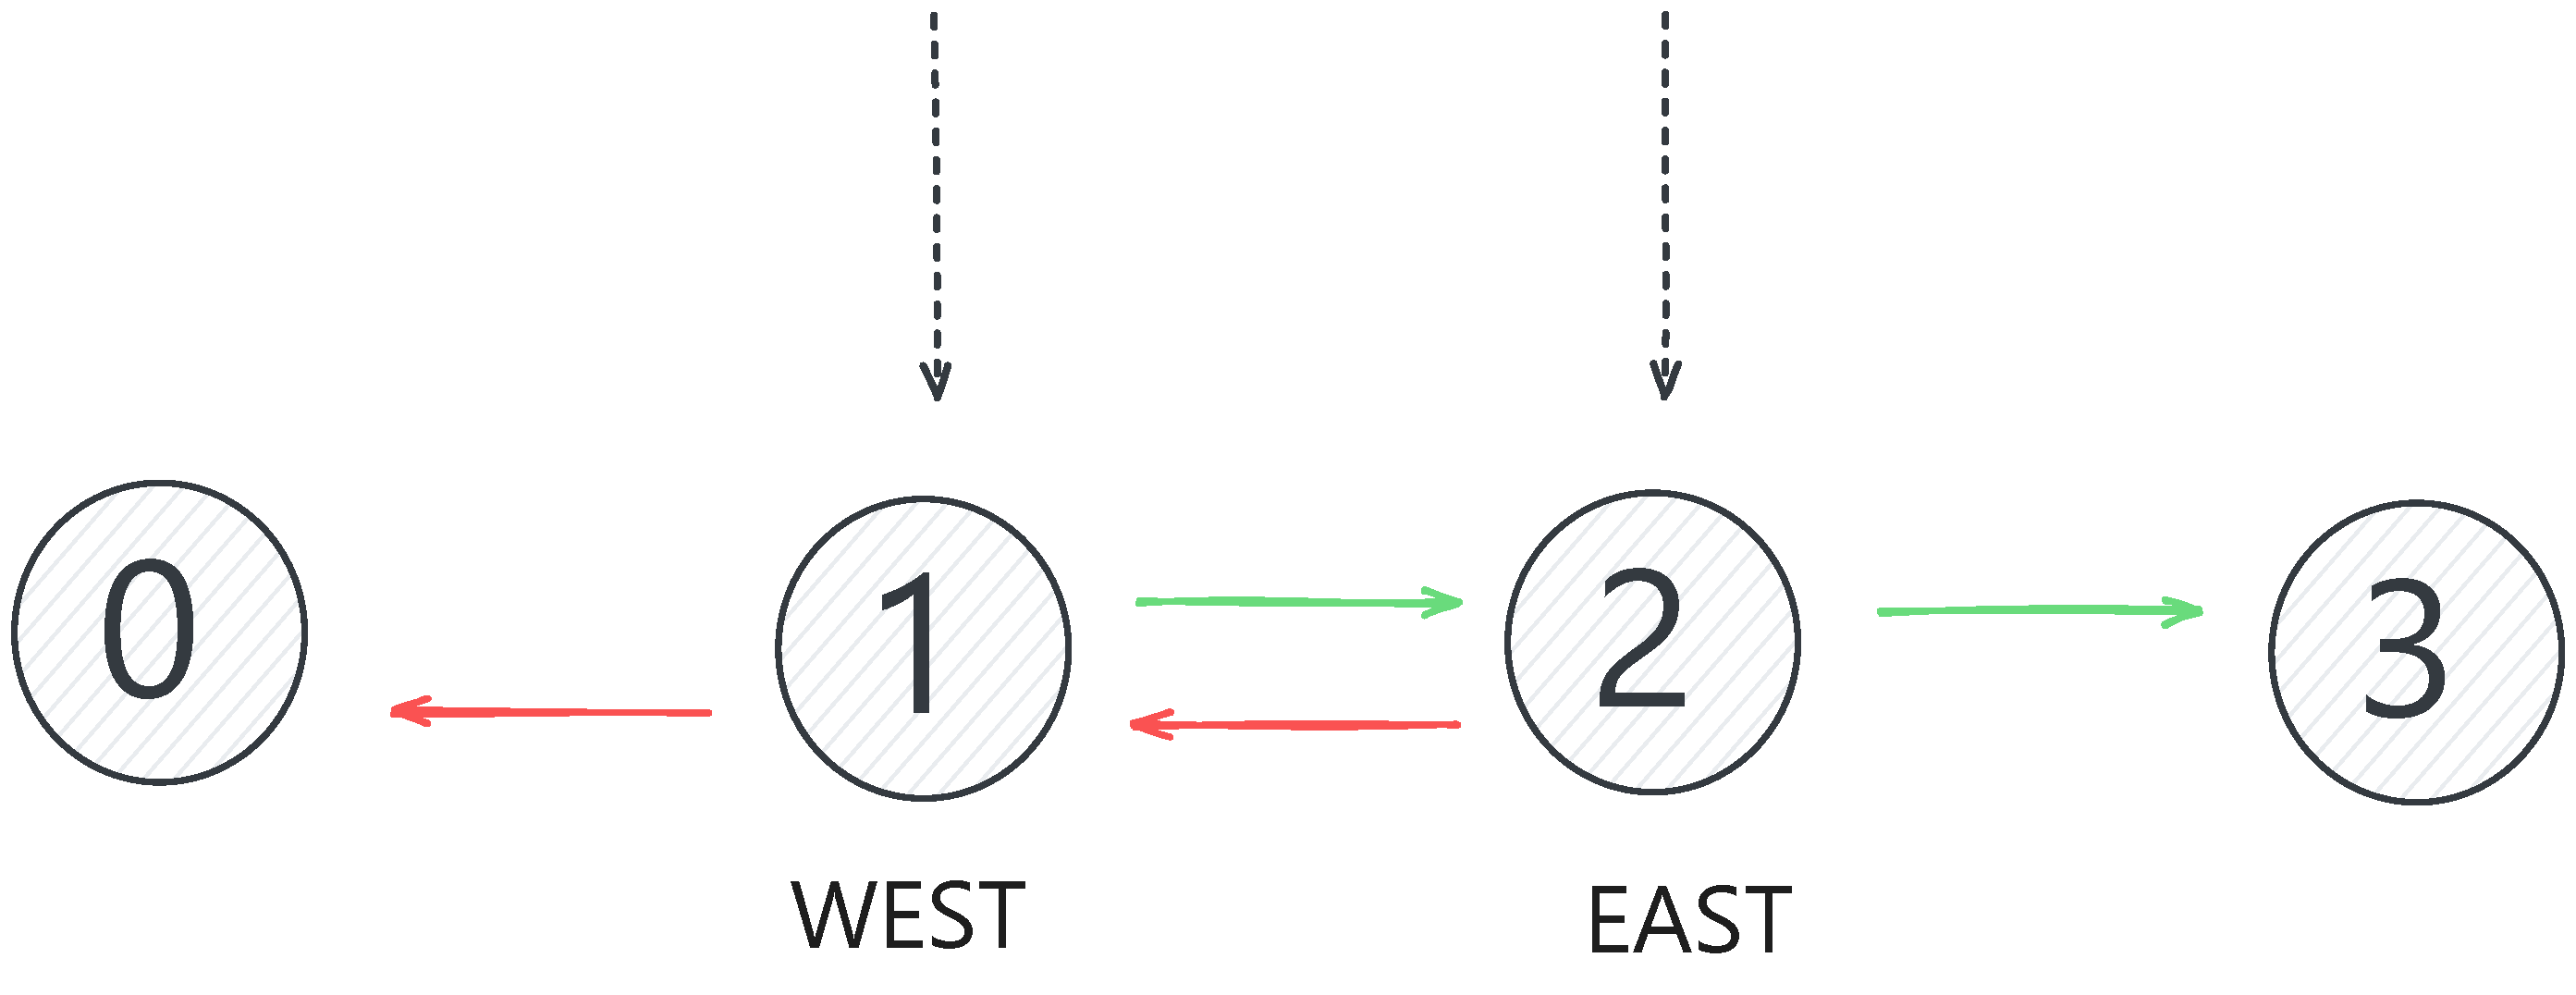
\includegraphics[width=0.5\linewidth]{plots/east_west_routing.pdf}
	\caption{Routing policy in example 7.}
	\label{fig:pdfimage}
\end{figure}


%\begin{figure}[h]
%	\centering
%	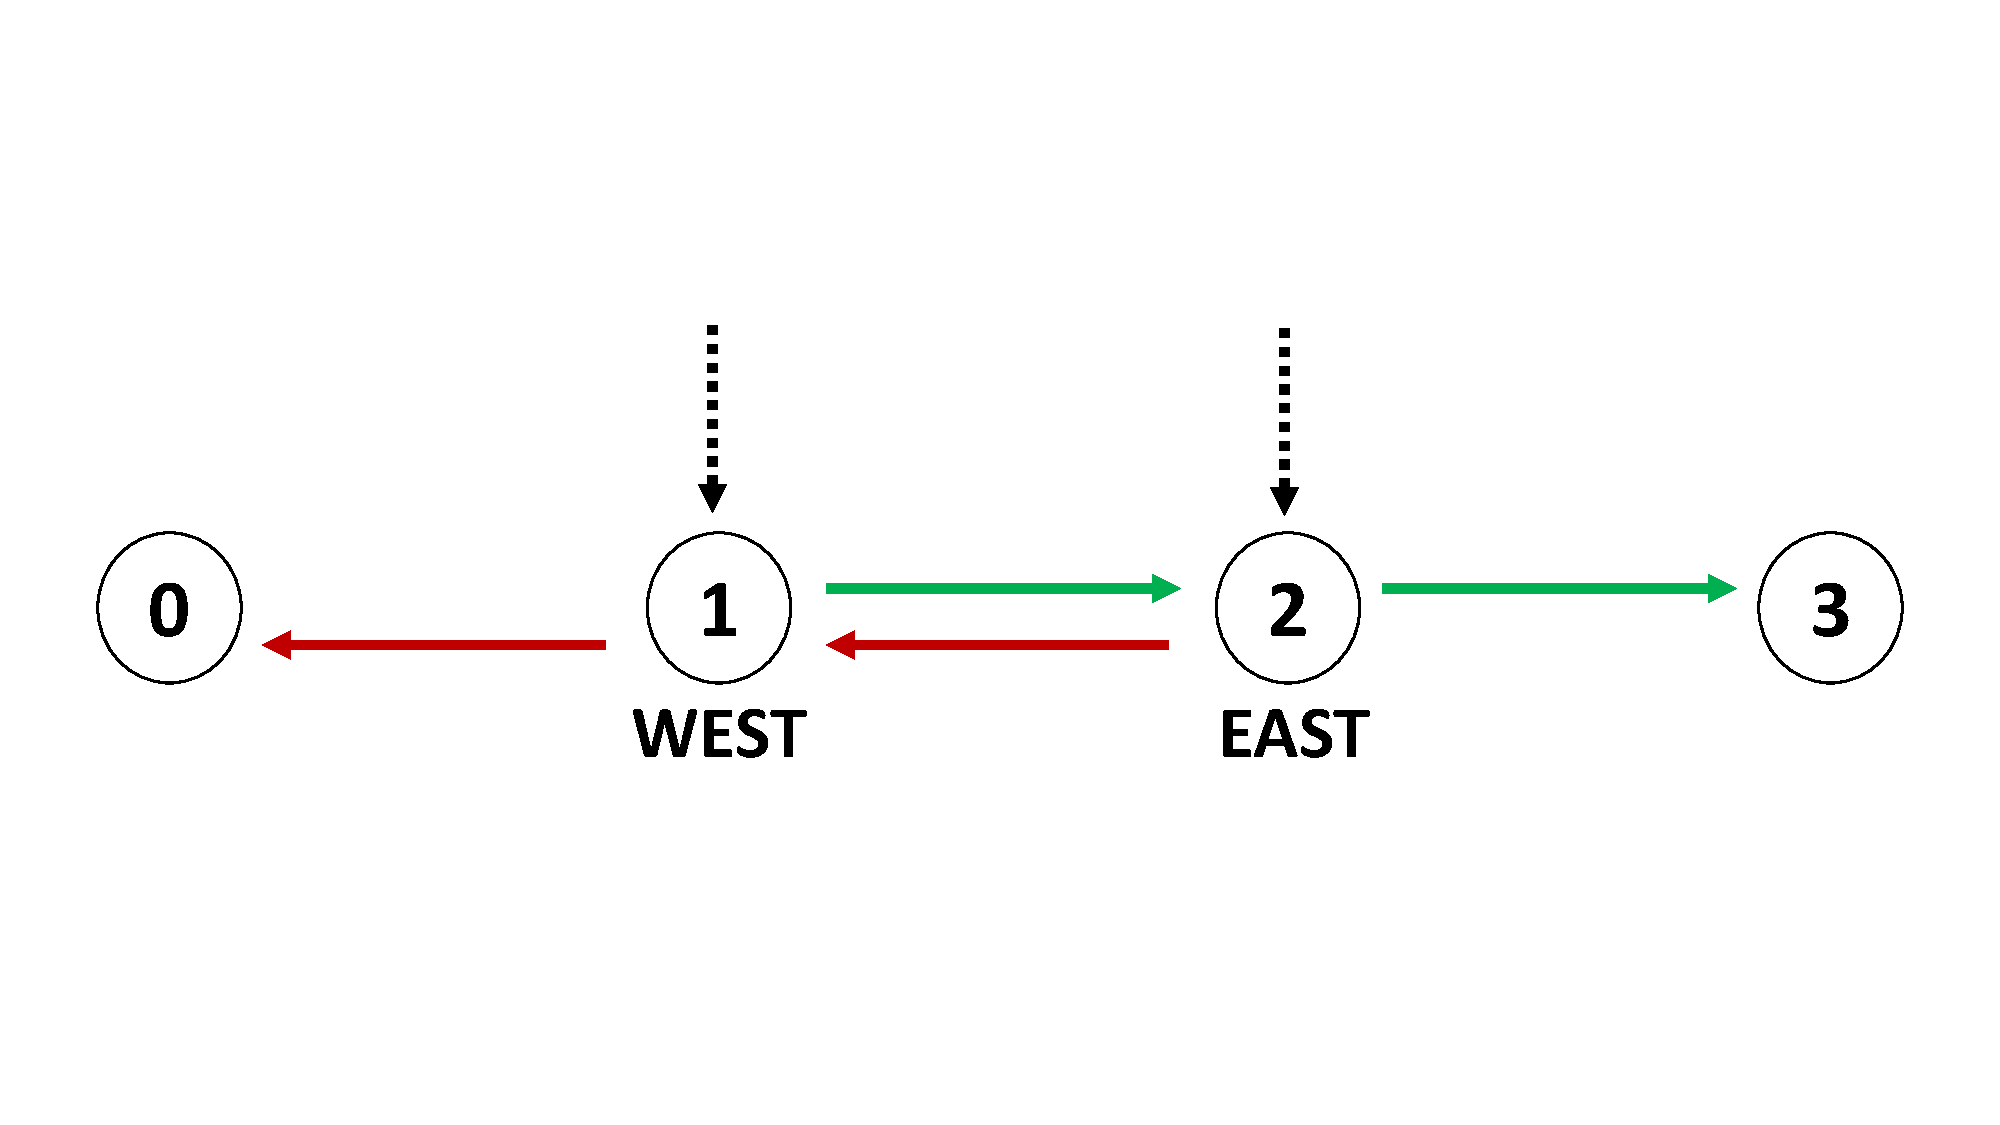
\includegraphics[width=0.65\linewidth]{plots/BgpColoredRouting.pdf}
%	\caption{Routing policy in example 7.}
%	\label{fig:pdfimage}
%\end{figure}

\newpage


example – 8

\noindent
\begin{minipage}[t]{0.45\textwidth}
	\begin{lstlisting}[caption={foo (serializable)}]
	request foo: 
	    if (?):
	        X := (X + 2) % 3 
	        // no yield
	        return X
	
	    else:
	        X := (X + 1) % 3
	        // no yield
	        return X
		\end{lstlisting}
\end{minipage}
\hfill
\begin{minipage}[t]{0.45\textwidth}
\begin{lstlisting}[caption={foo (non serializable)}]
request foo: 
     if (?):
         X := (X + 2) % 3 
         yield
         return X

     else:
         X := (X + 1) % 3
         yield
         return X
	\end{lstlisting}
\end{minipage}

One output that is attainable only via non-serializable executions is 
\[
\{(foo,1),(foo,1),(foo,1),(foo,3)\}
\]


%\newpage


example – 9

\noindent
\begin{minipage}[t]{0.45\textwidth}
	\begin{lstlisting}[caption={foo (serializable)}]
request foo:
    if(STOP == 0):
        X := (X + 1) % 4

    yield

    if(STOP == 0):
        X := (X + 1) % 4

        STOP := ?
        
        if(STOP == 1):
	        return X
        return 0
	\end{lstlisting}
\end{minipage}
\hfill
\begin{minipage}[t]{0.45\textwidth}
	\begin{lstlisting}[caption={foo (non serializable)}]
request foo:
    if(STOP == 0):
        X := (X + 1) % 4

    yield

    if(STOP == 0):
        X := (X + 2) % 4

        STOP := ?
        
        if(STOP == 1):
	        return X
        return 0
	\end{lstlisting}
\end{minipage}


